
%(BEGIN_QUESTION)
% Copyright 2011, Tony R. Kuphaldt, released under the Creative Commons Attribution License (v 1.0)
% This means you may do almost anything with this work of mine, so long as you give me proper credit

In this system, an Allen-Bradley SLC 500 PLC acts as a temperature controller, turning a cooling water solenoid valve on and off to modulate water flow to the heat-exchange jacket of a chemical reactor vessel.  A thermocouple monitors the temperature of the fluids within the vessel.  This diagram shows only the electrical connections (no piping, no other components represented) for simplicity:

$$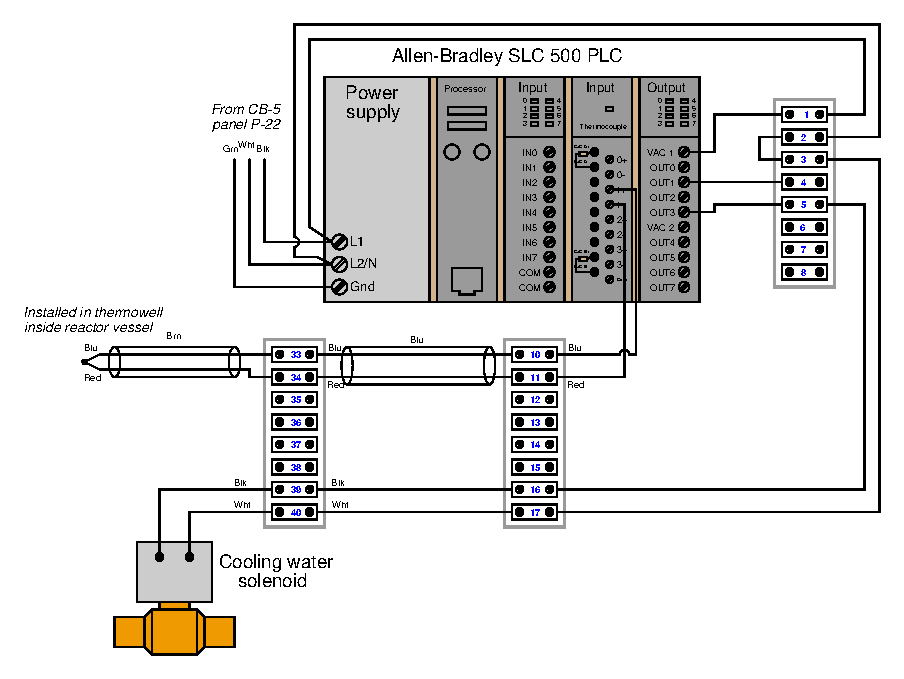
\includegraphics[width=15.5cm]{i03112x01.eps}$$

One day the operator of this reactor contacts you to say the reactor is overheating, based on the indication of a temperature gauge installed in the reactor near the PLC's thermocouple.  The reactor temperature high/low setpoint values programmed in the PLC are 85 deg C and 80 deg C, respectively.  The temperature gauge is registering 91 deg C and slowly climbing.

\vskip 10pt

Identify some likely faults that could cause this situation to occur, and also identify what tests you would begin to conduct in order to diagnose the problem.

\underbar{file i03112}
%(END_QUESTION)





%(BEGIN_ANSWER)

Possible faults include (but are not limited to):
 
\begin{itemize}
\item{} PLC program halted (with output {\tt O:3/3} stuck in the ``off'' state)
\item{} Discrete output {\tt O:3/3} channel bad (open TRIAC)
\item{} Short-circuit in thermocouple cable, causing it to register ambient temperature (low)
\item{} Failed thermocouple input {\tt I:2.1} channel, registering low temperature
\item{} 120 VAC power to PLC failed (e.g. breaker CB-5 tripped)
\item{} Cooling water supply failed
\item{} Solenoid valve stuck shut
\item{} Open wire fault between solenoid valve and PLC output card
\end{itemize}

%(END_ANSWER)





%(BEGIN_NOTES)


%INDEX% PLC, troubleshooting: temperature control system (thermocouple input card)

%(END_NOTES)


